\scanpage{100}
% archive foliation: 99
\deleted{Il y a un s-groupe d'indice fini\inserted{$I'$} de \deleted{$\unsure{\Pi|\pi}_1(U)$}\inserted{$I$} qui opère sur $E$ via un pro-$\ell$-groupe. À fortiori,}
\deleted{\diagram{\begin{tikzcd}
I_0(\deleted{\unsure{\bar\xi}}) \arrow[r] \arrow[d] & I'_0 \arrow[d] \\
I(\deleted{\unsure{\bar\xi}}) \arrow[r] & I'
\end{tikzcd}}}

\figure{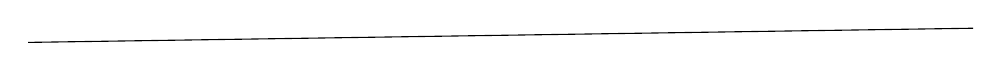
\begin{tikzpicture}[x=1cm,y=1cm]
\draw (0,0)--(12,.18);
\end{tikzpicture}}

\textcircled{a} Un résultat\inserted{local} de Abhyankar $\oplus$

\textcircled{b} \uline{Version \inserted{semi}globale du \deleted{\unsure{un}} résultat de Abhyankar}.

$X$ schéma loc. \unsure{n.th.} connexe

$\unsure{D}=\sum\unsure{D_i}$ diviseur\inserted{strictement} à croisements normaux

(composantes $Y_i$ \uline{régulières})

On suppose $Z=\bigcap_i\unsure{D_i}\ne\varnothing$, et que \deleted{\unsure{pour tt}}\inserted{le couple $(X,Z)$ est ``hensélien'', i.e. \unsure{pour} $\forall X'$ fini\inserted{sur $X$, conn $\ne\varnothing$}, \deleted{\unsure{l'image inverse} de $Z$ dans $X'$, $\unsure{\Pi|\pi}_0(\unsure{Z'})\simeq\unsure{\Pi|\pi}_0(X')$} $Z'$ est connexe $\ne\varnothing$}

\margin{\figure{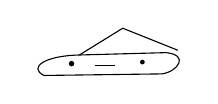
\begin{tikzpicture}[x=1cm,y=1cm]
\draw (0,.05) .. controls (-.2,.15) and (0,.3) .. (.45,.31) -- (1.55,.34) .. controls (1.85,.31) and (1.7,.1) .. (1.5,.07) -- cycle;
\fill (.35,.2) circle (.035); \fill (1.25,.22) circle (.03);
\draw (.65,.18)--(.9,.18);
\draw (.45,.31)--(1,.65)--(1.7,.37);
\end{tikzpicture}}}

\deleted{Alors} Soit \deleted{$\unsure{X}$} $U=X-\deleted{\unsure{supp}}Y$, $\xi$ un pt géom de $U$.

Alors a) $U$ connexe, et $\unsure{\Pi|\pi}_1(U,\xi)_t\longrightarrow\unsure{\Pi|\pi}_1(X,\xi)$ surjectif.

b) Pour tout $\unsure{D_i}$, le groupe d'inertie dans $\unsure{\Pi|\pi}_1(U,\xi)_t$ relatif \unsure{:|à} $\unsure{\Pi|\pi}_1(U)$ est un sous-groupe distingué \deleted{de $\unsure{\Pi|\pi}_1(U)\unsure{,\xi}$} commutatif $I_i$ de $Y_i$, \deleted{\unsure{on a}} et on a un épimorphisme canonique
\[
\deleted{\unsure{\xi}}
\prod_{\substack{\ell\ \text{inversible}\\\text{sur }\deleted{Z}\unsure{D_i}\\(\text{ou encore sur }Z)}}T_\ell(\Omega^*)\longrightarrow I_i.
\]

c) Les groupes $I_i$ commutent, et le \deleted{produit}\inserted{groupe engendré} est le noyau\inserted{$I$} de $\unsure{\Pi|\pi}_1(U,\xi)_t\unsure{-|\longrightarrow}\unsure{\Pi|\pi}_1(X,\xi)$.

a) Est immédiat.

b) L'image inverse de $\unsure{D_i}$ dans un rec. \deleted{\unsure{fini}}\inserted{connexe} \unsure{normal} modérément ramifié $X'$ de $X$ est normale (étude locale) et \uline{connexe}, \deleted{donc $I_i$ est} \unsure{irred}, donc $I_i$ est invariant. On sait bien qu'il est $\simeq$ quotient de $\prod_\ell T_\ell(\Omega^*)$, $\ell\ne\text{car. gén.}\text{ de }\unsure{D_i}$. Il faut prouver que $I$ est premier aux car. résiduelles en $\unsure{D_i}$. C'est une histoire locale sur $\unsure{D_i}$.

c) Commutation des $I_i$: \deleted{\unsure{Et.}} Étude locale en un pt de
